\tikzstyle{block} = [rectangle, minimum width=2cm, minimum height=1cm,text centered, draw=black]
\tikzstyle{block_1} = [rectangle, minimum width=2cm, minimum height=1cm,text centered, draw=black, fill=blue!5]
\tikzstyle{block_2} = [rectangle, minimum width=2cm, minimum height=1cm,text centered, draw=black, fill=red!5]
\tikzstyle{arrow} = [thick,->,>=stealth]
\tikzstyle{arrow_2} = [very thick,->,>=stealth, draw=blue]
\tikzstyle{arrow_3} = [thick,->,>=stealth,dashed]
\tikzstyle{pfr} = [cylinder, draw, minimum height=4cm, minimum width=1cm, shape aspect=1, shape border rotate=180]
\usetikzlibrary{shapes.geometric, calc}


\newpage
\section*{FIGURES}

\begin{figure}[!htbp]
    \centering
    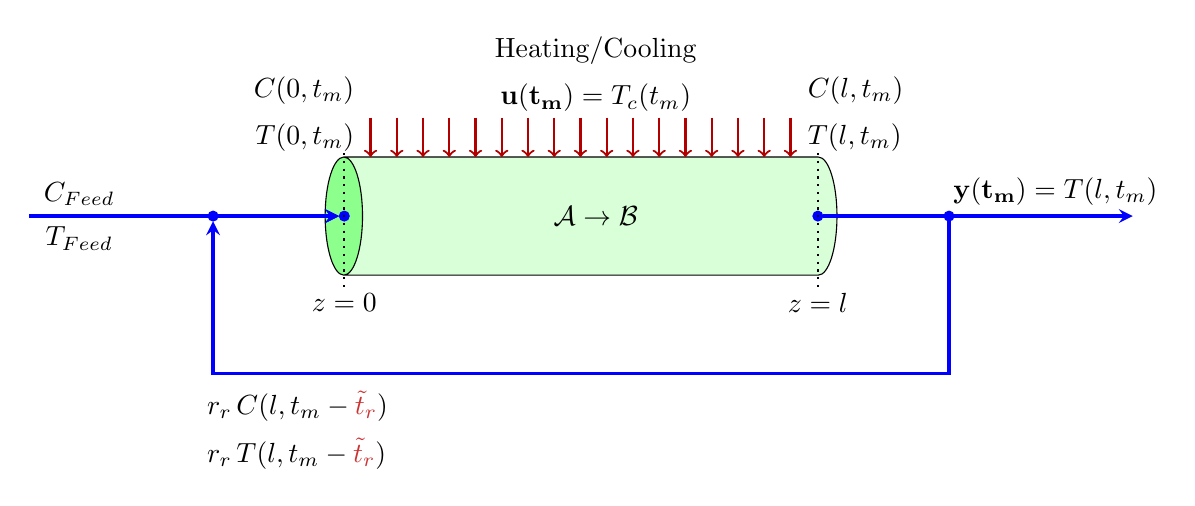
\begin{tikzpicture}
        \node (pfr) [cylinder, draw, minimum height=6.5cm, minimum width=1.5cm, shape aspect=1, shape border rotate=180, cylinder uses custom fill, cylinder end fill=green!45, cylinder body fill=green!15] {$\mathcal{A} \rightarrow \mathcal{B}$};
        \node (pfr_inlet) [circle, at={(pfr.west)}, shift={(0.25cm,0)}, fill=blue, draw=blue, inner sep=0pt, minimum size=0.25cm, scale=0.5] {};
        \node (pfr_outlet) [circle, at={(pfr.east)}, shift={(-0.25cm,0)}, fill=blue, draw=blue, inner sep=0pt, minimum size=0.25cm, scale=0.5] {};
        \node (recycle_right) [circle, at={(pfr_outlet.east)}, shift={(1.6cm,0)}, fill=blue, draw=blue, inner sep=0pt, minimum size=0.25cm, scale=0.5] {};
        \node (recycle_left) [circle, at={(pfr_inlet.west)}, shift={(-1.6cm,0)}, fill=blue, draw=blue, inner sep=0pt, minimum size=0.25cm, scale=0.5] {};

        \draw[dotted, thick] ([yshift=0.8cm]pfr_inlet.center) -- node[at end, below, yshift=0.1cm] {$z = 0$} ([yshift=-0.95cm]pfr_inlet.center);
        \draw[dotted, thick] ([yshift=0.8cm]pfr_outlet.center) -- node[at end, below, yshift=0.1cm] {$z = l$} ([yshift=-0.95cm]pfr_outlet.center);

        \node[below of=recycle_left, node distance=2.10cm, anchor=north west, xshift=-0.2cm] {$r_r \, C(l, t_m - \textcolor{red!60!gray}{\boldsymbol{\tilde{t}_r}})$};
        \node[below of=recycle_left, node distance=2.70cm, anchor=north west, xshift=-0.2cm] {$r_r \, T(l, t_m - \textcolor{red!60!gray}{\boldsymbol{\tilde{t}_r}})$};
        \node[above of=pfr_inlet, anchor=south east, node distance=1.30cm, xshift=0.25cm] {$C(0, t_m)$};
        \node[above of=pfr_inlet, anchor=south east, node distance=0.70cm, xshift=0.25cm] {$T(0, t_m)$};
        \node[above of=pfr_outlet, anchor=south west, node distance=1.30cm, xshift=-0.25cm] {$C(l, t_m)$};
        \node[above of=pfr_outlet, anchor=south west, node distance=0.70cm, xshift=-0.25cm] {$T(l, t_m)$};

        \draw [arrow_2] (pfr_outlet) -- node[near end, above] {$\mathbf{y(t_m)} = T(l, t_m)$} ++(4,0);
        \draw [arrow_2] (pfr_inlet) ++(-4,0) coordinate(start) -- node[near start, above, shift={(-0.35cm,0)}] {$C_{Feed}$} (pfr_inlet);
        \draw [arrow_2] (pfr_inlet) ++(-4,0) coordinate(start) -- node[near start, below, shift={(-0.35cm,0)}] {$T_{Feed}$} (pfr_inlet);
        \draw [arrow_2] (recycle_right) -- ++(0,-2.0) -| (recycle_left);

% Heat exchange arrows (from 1.5cm to 1.0cm above reactor)
        \foreach \i in {1,...,17} {
            \draw[->, red!70!black, thick] 
                ($([yshift=1.25cm]pfr_inlet.center) + (0.3333 * \i cm, 0)$) 
                -- 
                ($([yshift=0.75cm]pfr_inlet.center) + (0.3333 * \i cm, 0)$);
        }
        \node[anchor=south, yshift=1.2cm] at (pfr.center) {$\mathbf{u(t_m)} = T_c(t_m)$};
        \node[anchor=south, yshift=1.8cm] at (pfr.center) {Heating/Cooling};

    \end{tikzpicture}
    \caption{Non-isothermal axial dispersion tubular reactor with recycle stream.}
    \label{fig:reactor_scheme}
\end{figure}

\begin{figure}[!htbp]
    \centering
    \includesvg[inkscapelatex=false, width=1.0\textwidth, keepaspectratio]{Figures/steady_state_I.svg}
    \caption{Steady-state solutions for Case I. Solid and dashed lines represent reactor and recycle stream profiles, respectively.}
    \label{fig:ss_profiles}
\end{figure}

\begin{figure}[!htbp]
    \centering
    \includesvg[inkscapelatex=false, width=1.0\textwidth, keepaspectratio]{Figures/steady_state_II.svg}
    \caption{Steady-state solution for Case II. Solid and dashed lines represent reactor and recycle stream profiles, respectively.}
    \label{fig:ss_profiles_stable}
\end{figure}

\begin{figure}[!htbp]
    \centering
    \includesvg[inkscapelatex=false, width=1.0\textwidth, keepaspectratio]{Figures/eigenvalue_distribution_filtered.svg}
    \caption{Eigenvalue distribution in the complex plane for Case I (Unstable) and Case II (Stable).}
    \label{fig:eigvals}
\end{figure}

\begin{figure}[!htbp]
    \centering
    \includesvg[inkscapelatex=false, width=1.0\textwidth, keepaspectratio]{Figures/openloop_x.svg}
    \caption{3D profile of the state $x(\zeta, t)$ evolution over space and time $(\zeta, t)$ for Case I system with zero input.}
    \label{fig:openloop_x}
\end{figure}

\begin{figure}[!htbp]
    \centering
    \includesvg[inkscapelatex=false, width=0.6\textwidth, keepaspectratio]{Figures/input_output_MPC.svg}
    \caption{Profiles of plant output $y(t)$ and control input $u(t)$ over time for Case I system with full-state feedback MPC.}
    \label{fig:input_output_MPC}
\end{figure}

\begin{figure}[!htbp]
    \centering
    \includesvg[inkscapelatex=false, width=1.0\textwidth, keepaspectratio]{Figures/MPC_x.svg}
    \caption{3D profile of the state $x(\zeta, t)$ evolution over space and time $(\zeta, t)$ for Case I system with full-state feedback MPC.}
    \label{fig:MPC_x}
\end{figure}

\begin{figure}[!htbp]
    \centering
    \includesvg[inkscapelatex=false, width=1.0\textwidth, keepaspectratio]{Figures/input_output_MHE.svg}
    \caption{Profiles of plant output $y(t)$ and estimated output $\hat{y}(t)$ (left), and control input $u(t)$ (right) over time for Case II system with output feedback MHE-MPC.}
    \label{fig:input_output_MHE}
\end{figure}

\begin{figure}[!htbp]
    \centering
    \includesvg[inkscapelatex=false, width=1.0\textwidth, keepaspectratio]{Figures/MHE_x_true.svg}
    \caption{3D profile of the true state $x(\zeta, t)$ over time for Case II system with output feedback MHE-MPC.}
    \label{fig:MHE_x_true}
\end{figure}

\begin{figure}[!htbp]
    \centering
    \includesvg[inkscapelatex=false, width=1.0\textwidth, keepaspectratio]{Figures/MHE_x_est.svg}
    \caption{3D profile of the estimated state $\hat{x}(\zeta, t)$ over time for Case II system with output feedback MHE-MPC.}
    \label{fig:MHE_x_estimated}
\end{figure}

\begin{figure}[!htbp]
    \centering
    \includesvg[inkscapelatex=false, width=1.0\textwidth, keepaspectratio]{Figures/MHE_err.svg}
    \caption{3D profile of the state estimation error $e(\zeta, t) = x(\zeta, t) - \hat{x}(\zeta, t)$ over time for Case II system with output feedback MHE-MPC.}
    \label{fig:MHE_err}
\end{figure}

